\begin{figure*}
    \centering
    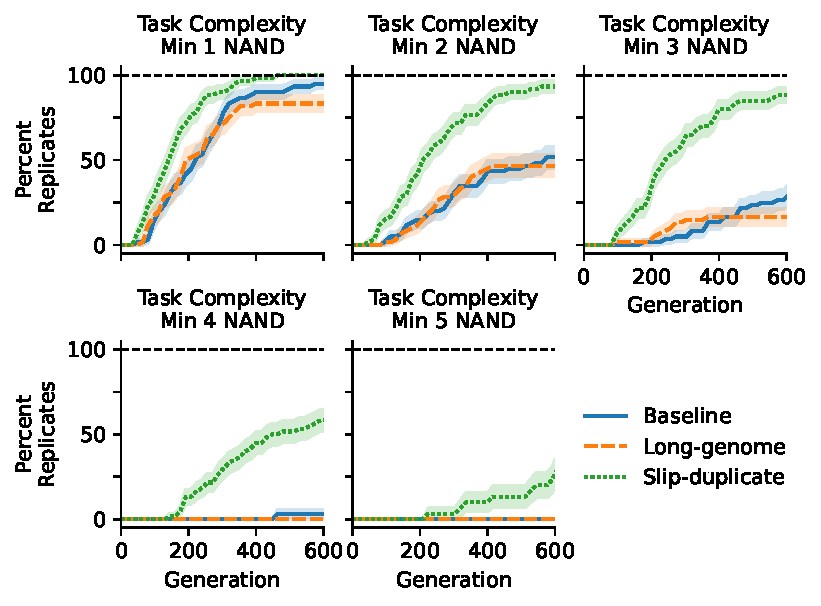
\includegraphics[width=\linewidth]{binder/binder/teeplots/adaptive-evolution-rate.ipynb/col=task-complexity+errorbar=se+hue=treatment+kind=line+mutation=poisson+post=plt-xlim-0-600+style=treatment+viz=relplot+x=generation+y=has-task+ext=.pdf}
    \caption{
        \textbf{Rate of adaptive evolution across a spectrum of task complexities, Poisson-distributed mutation.}
        \footnotesize
        Simple tasks (leftmost panels) require only one logic gate component.
        More complex tasks (rightmost panels) require up to five logic gate components.
        Compared to Figure \ref{fig:adaptive-evolution-rate}, which shows results with per-site mutation rates, the relative rate of adaptive evolution in long-genome control is diminished under Poisson-distributed treatment, where mutation count is not proportional to genome length.
        Error bands give 95\% CI, bootstrapped over 30 replicates per treatment.
    }
    \label{fig:adaptive-evolution-rate-poisson}
\end{figure*}
